\chapter{Vibration-based Damage Identification on system/structures modeled with NASTRAN, and using \textit{in silico} data}
\label{chp:8}
\epigraph{In theory, theory and practice are the same. \\In practice, they’re not.}{Yogi Berra}

\lstset{language=NASTRAN}
\lstset{keywords={GRID,GRDSET,SPC,DLOAD,DAREA,EIGRL,DELAY,CBAR,PBAR,PARAM,MAT1,CELAS2,CROD,MAT1,CONM2,TSTEP,TLOAD1,TLOAD2,TIC,TABDMP1}, keywordstyle={\color{blue!80!black}}}
\lstset{basicstyle=\scriptsize\ttfamily,breaklines=true}

In the last chapter, the defined methodology was applied in the damage identification of structures with models implemented in FORTRAN.

In this chapter, will be defined the experimental design for damage identification of structures with models in NASTRAN. Next, some case studies will be presented: a 2-DOF model, a 10-DOF model, a cantilevered truss, and a cantilevered beam.

\section{Experiment design}

The proposed damage identification approach takes the NASTRAN as the simulator of the structural model, and the hybrid metaheuristics as optimizer, as shown in \autoref{fig:inversenastran}.

The experiment design for identifying damages with structures modeled in NASTRAN consist of the following steps:

\begin{enumerate}[label=(\arabic*)]
    \item Create the NASTRAN input file of the structure, using the solution 109 (direct solution) or 112 (modal solution).
    \item Create \textit{in silico} observed data $u^{obs}$ using the damage configuration as input of the model, \textit{i.e.} modifying the stiffness of each damaged element.
    \item Add some noise to the synthetic measurements.
    \item Set-up the hybrid algorithm depending on the characteristics of the structure (dimension number, magnitude of the error, etc.).
    \item Run the hybrid algorithm at least 15 times, and tabulate the output damage parameters.
    \item Obtain some statistics, depending on the analysis to be performed.
\end{enumerate}

The main program modifies the NASTRAN input file. The stiffness values must be written in the appropriate element position with the correct format. Then the \texttt{nastran} application is called, to simulate the performance of the structure with the stiffness values configured. The NASTRAN return the requested data (such as displacement, frequency response, modal data) written in a punch file. In the next step, the program takes the computed model response, and compares it with the experimentally measured response.

\begin{figure}[H]
    \caption{Vibration-Based Damage Identification as optimization problem using NASTRAN as a black-box model}
    \label{fig:inversenastran}
    \centering
    \vspace{1em}
    \resizebox{0.8\textwidth}{!}{\includegraphics{images/chapter6_inversesolution.tikz}}
\end{figure}

\section{Case Study 1: Two-DOF Model}
\label{sec:twodof}

The approach is tested over a spring-mass system with 2-DOF, as shown in  \autoref{fig:twodof}. In this system, $k_{1} = 100 N/m$, $k_{2} = 1000 N/m$, $m_{1} = 0.1kg$ and $m_{2} = 10kg$. An external force $F(t) = 200N$ is applied over the element $m_2$.

\begin{figure}[H]
\caption{Case study 1: Spring mass system with 2-DOF}
\label{fig:twodof}
\centering
% \resizebox{\columnwidth}{!}{
\includegraphics{images/chapter6_twodof.tikz}
% }
\end{figure}

The NASTRAN input file modeling the system is shown in \autoref{lst:twodof}

\begin{lstlisting}[caption={NASTRAN input file for Two-DOF model},label={lst:twodof}]
$.......2.......3.......4.......5.......6.......7.......8.......9.......10.....$
TIC     777     2       2       0.1
TSTEP   888     1000    0.01    1    
GRID    1               0.      2.      0.
GRID    2               0.      1.      0.
GRID    3               0.      0.      0.
GRDSET                                                  13456
CONM2   1       1               0.1
CONM2   2       2               10.0 
CELAS2  11      100.0   1       2       2       2
CELAS2  12      1.0E4   2       2       3       2
SPC     996     3       2
\end{lstlisting}

It was set an initial displacement of $0.1~m$ at grid 2. The integration time step was set in $\Delta t = 0.01~s$, with a total integration time $t = 10~s$. Damping was assumed as negligible.

For the experiments, the optimization algorithm should modify the third column in the \texttt{CELAS2} cards which represent each spring in the system. That column represents the stiffness of the scalar spring.

\begin{figure}[H]
\caption{Damage identification on the spring-mass system}
\label{fig:resultspringmass2}
\centering
\begin{tikzpicture}
\begin{axis}[
        ybar,   
        width=\textwidth,
        height=0.3\textheight,
        bar width=5pt,
        enlargelimits=0.05,
        xmin = 0.5,
        xmax = 2.5,
        ymin = 0,
        ymax = 30,
        ymajorgrids,
        xminorgrids={true},
        minor x tick num=1,
        major grid style={line width=.2pt,draw=gray!50},
        minor grid style={line width=.2pt,draw=gray!50, dashed},
        ylabel={$\Theta^{\rm d}$},
        ylabel shift = 1 pt,
        xlabel={\footnotesize Element},
        xtick=data,
        ytick={0,10,20,30,40},
        restrict y to domain*=-5:40,
        nodes near coords align={horizontal},
        every node near coord/.append style={
            yshift=3pt,
            rotate=90,
            font=\tiny,
            xshift=-3pt,
            yshift=0pt,
            /pgf/number format/fixed
        },
        every axis y label/.style={
            at={(ticklabel* cs:1.05)},
            anchor=south,
        },
        every axis/.append style={
            font=\scriptsize
        },
        legend entries={Damage, RBSMPCA-HJ, $q$G-HJ},
        legend columns=5,
        legend style={draw=none,font=\scriptsize},
        legend style={fill=none},
        legend pos= {north west}
    ]
\addplot [draw,
         fill=white,
         nodes near coords=\pgfmathprintnumber{\pgfplotspointmeta},
         /pgf/number format/precision=1]
	coordinates {(1,20)	(2,20)};
\addplot [draw,
         fill=yaleblue,
         nodes near coords=\pgfmathprintnumber{\pgfplotspointmeta},
         /pgf/number format/precision=1]
	coordinates {(1,20) (2,20)};
\addplot [draw,
         fill=oucrimsonred,
         nodes near coords=\pgfmathprintnumber{\pgfplotspointmeta},
         /pgf/number format/precision=1]
	coordinates {(1,20) (2,20)};
\end{axis}
\end{tikzpicture}
\end{figure}

\section{Case Study 2: Ten-DOF Model}
\label{sec:tendof}

The results in this section were presented in the Conference of Computational Interdisciplinary Science (CCIS 2016) - \cite{hernandez2016ccis}.

A spring-mass system with 10-DOF, as shown in  \autoref{fig:tendof}, is tested. In this case, $k_{1-9} = 100 N/m$, $k_{10} = 1000 N/m$, $m_{1-9} = 0.1kg$ and $m_{10} = 10kg$, and the system is excited with a external force $F(t) = 200N$ applied over the element $m_2$.

\begin{figure}[H]
\caption{Case study 2: Spring mass system with 10-DOF}
\label{fig:tendof}
\centering
\resizebox{\columnwidth}{!}{
\includegraphics{images/chapter6_tendof.tikz}
}
\end{figure}

A fragment of the NASTRAN input file that models the system is shown in \autoref{lst:tendof}. In the bulk data, the entries to be manipulated are those that begin with \texttt{CELAS2}, each one representing the springs in the system. The third column in the card represents the stiffness of the scalar spring.

\begin{lstlisting}[caption={NASTRAN input file for Ten-DOF model},label={lst:tendof}]
$.......2.......3.......4.......5.......6.......7.......8.......9.......10.....$
CELAS2  11      100     1       2       2       2
CELAS2  12      100     2       2       3       2
CELAS2  13      100     3       2       4       2
CELAS2  14      100     4       2       5       2
CELAS2  15      100     5       2       6       2
CELAS2  16      100     6       2       7       2
CELAS2  17      100     7       2       8       2
CELAS2  18      100     8       2       9       2
CELAS2  19      100     9       2       10      2
CELAS2  20      1000    10      2       11      2                                   \end{lstlisting}

\autoref{fig:resultspringmass10} shows the results of the damage identification with noiseless data graphically. Each separation in the graph box represents an element in the structure; the blue bars represent the value of the damage to be estimated, and the red bars represent the estimated damage parameters. In this case, results are almost perfect.

\begin{figure}[H]
\pgfplotstableread{%
    element 1 2 3 4 5 6 7 8 9 10
    damage 0 10 0 10 0 30 0 0 15 0 
    mpca 1.38    5.37    6.37    16.10    1.32    29.55    0.18    2.07    4.12    5.81
    rbs -0.08   9.98   0.09  10.17   0.14  -0.06  -0.21  -0.07  15.06   0.00
    }\datatable
    \pgfplotstabletranspose[colnames from=element]\dataset{\datatable}
    
\caption{Damage identification on the spring-mass system}
\label{fig:resultspringmass10}
\centering
\begin{tikzpicture}
\begin{axis}[
        ybar,   
        width=\textwidth,
        height=0.3\textheight,
        bar width=5pt,
        enlargelimits=0.05,
        xmin = 1,
        xmax = 10,
        ymin = 0,
        ymax = 30,
        ymajorgrids,
        xminorgrids={true},
        minor x tick num=1,
        major grid style={line width=.2pt,draw=gray!50},
        minor grid style={line width=.2pt,draw=gray!50, dashed},
        ylabel={$\Theta^{\rm d}$},
        ylabel shift = 1 pt,
        xlabel={\footnotesize Element},
        xtick=data,
        ytick={0,10,20,30,40},
        restrict y to domain*=-5:40,
        nodes near coords align={horizontal},
        every node near coord/.append style={
            yshift=3pt,
            rotate=90,
            font=\tiny,
            xshift=-3pt,
            yshift=0pt,
            /pgf/number format/fixed
        },
        every axis y label/.style={
            at={(ticklabel* cs:1.05)},
            anchor=south,
        },
        every axis/.append style={
            font=\scriptsize
        },
        legend entries={Damage, MPCA-HJ, RBMPCA-HJ},
        legend columns=5,
        legend style={draw=none,font=\scriptsize},
        legend style={fill=none},
        legend pos= {north east}
    ]
\addplot [draw,
         fill=yaleblue,
         nodes near coords=\pgfmathprintnumber{\pgfplotspointmeta},
         /pgf/number format/precision=1]
	coordinates {
	(1,0*100)
	(2,0*100)
	(3,0.10*100)
	(4,0.25*100)
	(5,0.15*100)
	(6,0*100)
	(7,0*100)
	(8,0.05*100)
	(9,0*100)
	(10,0*100)};
\addplot [draw,
         fill=oucrimsonred,
         nodes near coords=\pgfmathprintnumber{\pgfplotspointmeta},
         /pgf/number format/precision=1]
	coordinates {
	(1,(100-1.00000*100)
	(2,(100-0.99941*100)
	(3,(100-0.90020*100)
	(4,(100-0.75104*100)
	(5,(100-0.85102*100)
	(6,(100-1.00000*100)
	(7,(100-0.99991*100)
	(8,(100-0.95342*100)
	(9,(100-1.00000*100)
	(10,(100-1.00000*100)};
\end{axis}
\end{tikzpicture}
\end{figure}

\section{Case Study 3: Cantilever truss}
\label{sec:cantilevertruss}

The results in this section were presented in the 4th Conference of Computational Interdisciplinary Science (CCIS 2016) - \cite{hernandez2016ccis}.

The other case study is a cantilever truss \cite{VENKAYYA1971265} with 10 bars, as shown in \autoref{fig:cantilevertruss}. The structure configuration was taken from the NASTRAN Compatible Finite Elements (CoFE)\footnote{\scriptsize\url{http://vtpasquale.github.io/NASTRAN_CoFE/tenBarTrussOptimization.html}} \cite{ricciardi2015nonlinear}. The unit were converted to the International System of Units. In this structure, $L = 9.144 m$, $P = 444.82kN$, Young's modulus equal to $6.895 \times 10^{10} Pa$, and a specific mass equal to $27679,9 kg/m^3$, with a minimum area of $0,00064516m^2$.


In the case of the truss system, the NASTRAN entries to be manipulated are those that begin with \texttt{MAT1}, which represents the material of a single element, in this case a bar. Each line in \autoref{lst:ctruss} represents a single bar. The third column in the card represents the Young’s modulus, and this is the value modified in this case for representing the losses of stiffness.

\begin{lstlisting}[caption={NASTRAN input file for Cantilever Truss},label={lst:ctruss}]
$ 1-----2-------3-------4-------5-------6-------7-------8-------
MAT1    101     1.E7            .33     2.59E-4
MAT1    201     1.E7            .33     2.59E-4
MAT1    301     1.E7            .33     2.59E-4
MAT1    401     1.E7            .33     2.59E-4
MAT1    501     1.E7            .33     2.59E-4
MAT1    601     1.E7            .33     2.59E-4
MAT1    701     1.E7            .33     2.59E-4
MAT1    801     1.E7            .33     2.59E-4
\end{lstlisting}

\begin{figure}[H]
\caption{Case study 3: Two-bay truss structure}
\label{fig:cantilevertruss}
\centering
\resizebox{0.65\columnwidth}{!}{
\begin{tikzpicture}[node distance=1mm]

\clip(0,1) rectangle (8,5);
\coordinate (c) at (6,4);
\coordinate (d) at (6,2);
\coordinate (e) at (4,4);
\coordinate (f) at (4,2);
\coordinate (g) at (2,4);
\coordinate (h) at (2,2);

\node[hinge b,draw] (C) at (c){};
\node[hinge b,draw] (D) at (d){};
\node[hinge b,draw] (E) at (e){};
\node[hinge b,draw] (F) at (f){};
\node[hinge,draw,grounded=270,scale=0.85,transform shape] (G) at (g){};
\node[hinge,draw,grounded=270,scale=0.85,transform shape] (H) at (h){};

\draw[thick] (G)
-- node[sloped, above] {\footnotesize 1} (E)
-- node[sloped, above] {\footnotesize 2} (C)
-- node[sloped, above] {\footnotesize 6} (D)
-- node[sloped, below] {\footnotesize 4} (F)
-- node[sloped, below] {\footnotesize 3} (H)
-- node[sloped, above] {\hspace{2em}\footnotesize 8} (E)
-- node[sloped, above] {\footnotesize 5} (F)
-- node[sloped, above] {\hspace{2em}\footnotesize 10} (C)
;

\draw[thick] (G) -- node[sloped, above] {\hspace{2em}\footnotesize 7} (F);
\draw[thick] (E) -- node[sloped, above] {\hspace{2em}\footnotesize 9} (D);

\draw [-latex, thick , gray] (F) -- +(0,-0.7cm)
    node [midway, right] {\small $P$};
\draw [-latex, thick , gray] (D) -- +(0,-0.7cm)
    node [midway, right] {\small $P$};
    
%\draw[very thick,red] (5,7) -- (6,7) node[right] {damage};
% \draw[<->] (8,3.3) node[above] {\small $y$} -- (8,2.5) -- (8.8,2.5) node[below] {\small $x$};
% \draw [->] (8.75,2.75) node[sloped, left=0.15] {\small $+$} arc (0:90:0.5);
\end{tikzpicture}
}
\end{figure}

\quad

\begin{figure}[H]
\caption{Damage identification on the truss structure}
\label{fig:resulttruss}
\centering
\begin{tikzpicture}
\begin{axis}[
        ybar,   
        width=\textwidth,
        height=0.3 \textheight,
        bar width=5pt,
        enlargelimits=0.05,
        xmin = 1,
        xmax = 10,
        ymin = 0,
        ymax = 30,
        ymajorgrids,
        xminorgrids={true},
        minor x tick num=1,
        major grid style={line width=.2pt,draw=gray!50},
        minor grid style={line width=.2pt,draw=gray!50, dashed},
        ylabel={$\Theta^{\rm d}$},
        ylabel shift = 1 pt,
        xlabel={\footnotesize Element},
        xtick=data,
        ytick={0,10,20,30,40},
        restrict y to domain*=-5:40,
        nodes near coords align={horizontal},
        every node near coord/.append style={
            yshift=3pt,
            rotate=90,
            font=\tiny,
            xshift=-3pt,
            yshift=0pt,
            /pgf/number format/fixed
        },
        every axis y label/.style={
            at={(ticklabel* cs:1.05)},
            anchor=south,
        },
        every axis/.append style={
            font=\scriptsize
        },
        legend entries={Damage, MPCA-HJ, RBMPCA-HJ},
        legend columns=5,
        legend style={draw=none,font=\scriptsize},
        legend style={fill=none},
        legend pos= {north east}
    ]
\addplot[draw,
         fill=yaleblue,
         nodes near coords=\pgfmathprintnumber{\pgfplotspointmeta},
         /pgf/number format/precision=1]
	coordinates {
	(1,0*100)
	(2,0*100)
	(3,0.10*100)
	(4,0.25*100)
	(5,0.15*100)
	(6,0*100)
	(7,0*100)
	(8,0.05*100)
	(9,0*100)
	(10,0*100)};
\addplot[draw,
         fill=oucrimsonred,
         nodes near coords=\pgfmathprintnumber{\pgfplotspointmeta},
         /pgf/number format/precision=1] 
	coordinates {
	(1,(100-1.00000*100)
	(2,(100-0.98405*100)
	(3,(100-0.90185*100)
	(4,(100-0.82108*100)
	(5,(100-0.77502*100)
	(6,(100-0.99705*100)
	(7,(100-0.93921*100)
	(8,(100-0.98342*100)
	(9,(100-1.00000*100)
	(10,(100-0.98853*100)};
\end{axis}
\end{tikzpicture}
\end{figure}

\autoref{fig:resulttruss} shows the results of the damage identification with noiseless data. Again, each separation in the graph box represents an element in the structure; the blue bar represents the value of the damage to be estimated, and the red bar the damage identified. In this case, results are worst than in the spring-mass system. The damages in the $3^{rd}$, $4^{th}$ and $5^{th}$ elements were identified, but the method fails to estimate the damage severity. The damage located at the $8^{th}$ element was not correctly estimated, and in the $7^{th}$ element a false alarm appeared.

\section{Case Study 4: Cantilever beam}

\autoref{fig:beamnastran} shows a cantilever beam model. The beam has a length $\ell = 3m$, with a radius $r = 0.014m$, $J = 6.0\times10^{-8}m^4$, $A=6.158\times10^{-4}m^2$, $I1 = I2 = 3.0\times10^{-8}m^4$, the weight density $\rho_w = 2.65\times10^{4}N/m^3$, the Young' modulus $E = 7.1\times10^{10}N/m^2$, $\nu=0.33$, and has a nonstructural weight $= 2.414N/m$. This model come from the modified example in the \say{Chapter 6 - Transient Response Analysis} of the book \say{Basic Dynamic Analysis User's Guide} \cite{nastran2004basic}.

\begin{figure}[H]
\caption{Case study 4: Cantilever Beam structure}
\label{fig:beamnastran}
\centering
\includegraphics{images/chapter6_beam.tikz}
\end{figure}

The damage identification is performed using the modal transient response (SOL 112). Loads are applied to grids 5 and 10, as shown in \autoref{fig:beamnastranelements}. The waveform of each load is shown in \autoref{fig:loadsbeam} The analysis is run with a time step $\Delta t=0.001s$, and $t_f = 2s$. Modal damping of 5\% critical damping is used for all modes. Modes up to $3000Hz$ are computed using Lanczos method.

\begin{figure}[H]
\caption{Cantilever Beam with applied loads}
\label{fig:beamnastranelements}
\centering
\includegraphics{images/chapter6_beamelements.tikz}
\end{figure}

\begin{figure}[H]
\caption{Loads applied on the cantilever beam}
\label{fig:loadsbeam}
\centering
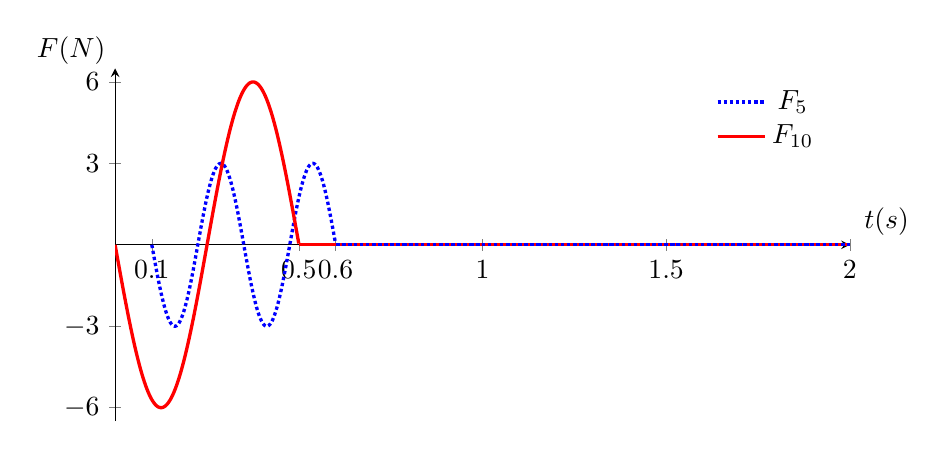
\begin{tikzpicture}
\begin{axis}[
    width=0.9\textwidth,
    height=0.5\textwidth,
    xmin=0,
    xmax=2,
    ymin=-6.5,
    ymax=6.5,
    axis lines=middle,
    xtick={0.1,0.5,0.6,1,1.5,2},
    ytick={-6,-3,3,6},
    xlabel=$t(s)$,
    ylabel=$F(N)$,
    legend columns=1,
    legend style={fill=none,draw=none},
    legend pos= {north east},
    every axis y label/.style={
            at={(ticklabel* cs:1.05)},
            anchor=east,
        },
    every axis x label/.style={
            at={(ticklabel* cs:1.05)},
            anchor=south,
        },
    every axis*/.append style={
            font=\scriptsize
        },
]
\addplot[samples=500,domain=0.1:0.6,densely dotted,blue,very thick] {-3*sin(25.1*deg(x-0.1))};\label{plot_one}
\addplot[samples=500,domain=0:0.5,red,very thick]   {-6*sin(12.55*deg(x))};\label{plot_two}
\addplot[samples=500,domain=0.5:2,red,very thick] {0};
\addplot[samples=500,domain=0.6:2,densely dotted,blue,very thick] {0};

\addlegendimage{/pgfplots/refstyle=plot_one}\addlegendentry{$F_5$}
\addlegendimage{/pgfplots/refstyle=plot_two}\addlegendentry{$F_{10}$}


\end{axis}
\end{tikzpicture}
\end{figure}

The weight density $\rho_w$ is converted to mass density $\rho_m$ for consistency of units. The entry \texttt{PARAM, WTMASS} is used for doing this conversion.
%
\begin{equation}
    \rho_m = \rho_w \cdot WTMASS    
\end{equation}
%
\begin{equation}
    WTMASS = 1/g = 1/9.81 = 0.102 s^2/m
\end{equation}
%
Then,
\begin{equation}
    \rho_m = 2.65\times10^{4}N/m^3 \cdot 0.102 s^2/m = 2703kg/m^3    
\end{equation}

The loads are set using the \texttt{DLOAD} entry, that references two \texttt{TLOAD2} entries. Each \texttt{TLOAD2} entry references a \texttt{DAREA}, and one of them (the one that defines the load applied at grid 6) references a \texttt{DELAY} entry.

% \lstinputlisting[caption={NASTRAN input file for Cantilever Beam},label={lst:cbeam}]{data/bd05bar.dat}

\begin{lstlisting}[caption={NASTRAN input file for Cantilever Beam},label={lst:cbeam}]
EIGRL   10      -0.1    3000.           0
TSTEP   27      2000    0.001   1
TABDMP1 25      CRIT                                                    +TABD
+TABD   0.      0.05    1000.   0.05    ENDT
DLOAD   22      1.0     1.0     231     1.0     232
TLOAD2  231     241             0       0.0     0.50    2.0     90.
TLOAD2  232     242     262     0       0.0     0.50    4.0     90.
DAREA   241     11      2       6.0
DAREA   242     6       2       3.0
DELAY   262     6       2       0.1
GRDSET                                                  345
MAT1    1       7.1+10          0.33    2.65+4
PARAM   WTMASS  0.102
PBAR    1       1       6.158-4 3.0-8   3.0-8   6.-8    2.414
CBAR    1       1       1       2       0.      1.      0.                      
CBAR    2       1       2       3       0.      1.      0.                      
CBAR    3       1       3       4       0.      1.      0.                      
CBAR    4       1       4       5       0.      1.      0.                      
CBAR    5       1       5       6       0.      1.      0.                      
CBAR    6       1       6       7       0.      1.      0.                      
CBAR    7       1       7       8       0.      1.      0.                      
CBAR    8       1       8       9       0.      1.      0.                      
CBAR    9       1       9       10      0.      1.      0.                      
CBAR    10      1       10      11      0.      1.      0.                      
GRID    1               0.0     0.      0.                                      
GRID    2               0.3     0.      0.                                      
GRID    3               0.6     0.      0.                                      
GRID    4               0.9     0.      0.                                      
GRID    5               1.2     0.      0.                                      
GRID    6               1.5     0.      0.                                      
GRID    7               1.8     0.      0.                                      
GRID    8               2.1     0.      0.                                      
GRID    9               2.4     0.      0.                                      
GRID    10              2.7     0.      0.                                      
GRID    11              3.0     0.      0.                                      
SPC     21      1       126
\end{lstlisting}

\begin{figure}[H]
\caption{Results for the MPCA-HJ and RBSMPCA-HJ on the case study 6 using a dataset few time series - Configuration with mixed damages}
\label{fig:cbeam}
\centering
\pgfplotstableread{%
    element 1 2 3 4 5 6 7 8 9 10
    damage 0 10 0 20 0 30 0 0 5 10 
    mpca 1.38    5.37    6.37    16.10    1.32    29.55    0.18    2.07    4.12    5.81
    rbs 1.31    5.75    5.28    17.55    0.65    29.72    0.07    1.02    5.80    5.32
    }\datatable
    \pgfplotstabletranspose[colnames from=element]\dataset{\datatable}
      
\begin{tikzpicture}
\begin{axis}[
        ybar,   
        width=\textwidth,
        height=0.3 \textheight,
        bar width=5pt,
        enlargelimits=0.05,
        xmin = 1,
        xmax = 10,
        ymin = 0,
        ymax = 40,
        ymajorgrids,
        xminorgrids={true},
        minor x tick num=1,
        major grid style={line width=.2pt,draw=gray!50},
        minor grid style={line width=.2pt,draw=gray!50, dashed},
        ylabel={$\Theta^{\rm d}$},
        ylabel shift = 1 pt,
        xlabel={\footnotesize Element},
        xtick=data,
        ytick={0,10,20,30,40},
        restrict y to domain*=-5:40,
        nodes near coords align={horizontal},
        every node near coord/.append style={
            yshift=3pt,
            rotate=90,
            font=\tiny,
            xshift=-3pt,
            yshift=0pt,
            /pgf/number format/fixed
        },
        every axis y label/.style={
            at={(ticklabel* cs:1.05)},
            anchor=south,
        },
        every axis/.append style={
            font=\scriptsize
        },
        legend entries={Damage, MPCA-HJ, RBMPCA-HJ},
        legend columns=5,
        legend style={draw=none,font=\scriptsize},
        legend style={fill=none},
        legend pos= {north west}
    ]
        
\addplot[draw=black,fill=white,nodes near coords=\pgfmathprintnumber{\pgfplotspointmeta},
        /pgf/number format/precision=1]
%plot [error bars/.cd, y dir = both, y explicit]
table[x index=0,y index=1] \dataset;
\addplot[draw=black,fill=yaleblue,nodes near coords=\pgfmathprintnumber{\pgfplotspointmeta},
        /pgf/number format/precision=1]
%plot [error bars/.cd, y dir = both, y explicit]
table[x index=0,y index=2] \dataset;
\addplot[draw=black,fill=armygreen,nodes near coords=\pgfmathprintnumber{\pgfplotspointmeta},
        /pgf/number format/precision=1]
%plot [error bars/.cd, y dir = both, y explicit]
table[x index=0,y index=3] \dataset;
\end{axis}
\end{tikzpicture}
\end{figure}

\section{Chapter conclusions}

